\section{Les relations positives et négatives}

Précédemment, les relations étudiées étaient considérées comme uniquement positives (on ne peut se faire que des amis). 

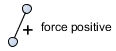
\includegraphics[scale=1]{images/22_force-positive}

Dans ce chapitre, nous allons étudier les graphes comportant également des relations positives et des relations négatives (on peut se faire des amis et des ennemis).

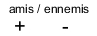
\includegraphics[scale=1]{images/22_amis-ennemis3.png}

\subsection{Théorie de l'équilibre de structure}
L'équilibre dans une structure va nous permettre d'identifier les situations stables et celles qui sont instables. Cette étude se fera dans un graphe complet (un graphe dont chaque paire a un lien et dont chaque lien peut être de type "+" ou "-").

\paragraph{}
L'idée cruciale est d'identifier dans le graphe les situations équilibrées et les situations qui ne le sont pas et qui engendrent un stress entre les nœuds.  

\begin{figure}[h!]
\label{equi}
\caption{Relations équilibrées et non équilibrées}
\centering
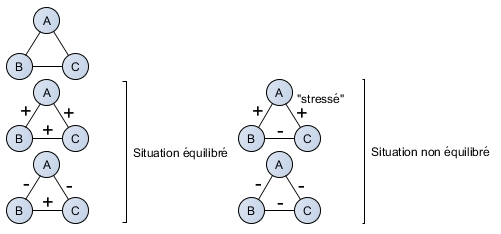
\includegraphics[width=\textwidth]{images/22_situation.png}
\end{figure}


Dans la figure \ref{equi}, les schémas de gauche sont considérés comme équilibrés. En effet, soit A, B et C sont tous amis et il n'y aucun conflit entre eux, soit B et C sont amis, mais sont en confit avec A. 
\paragraph{}
Par contre, les schémas de droite sont des situations non équilibrées. Dans la 3, B et C sont amis avec A mais ennemis entre eux, on peut supposer que A doive alors choisir un camp. La 4 indique que tous sont ennemis, mais il est fort probable que le graphe évolue vers une situation où deux nœuds se liguent contre le troisième. 

\paragraph{}
 
 On peut maintenant généraliser cela pour un nombre quelconque de nœuds. Ainsi un graphe complet sera équilibré si chaque ensemble de 3 nœuds est équilibré et donc possède des liens de type $+++$ ou $+--$.   

\begin{figure}[h!]
\label{equi2}
\caption{Généralisation des relations équilibrées et non équilibrées}
\centering
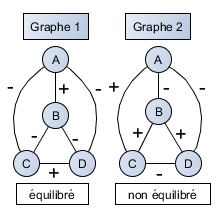
\includegraphics[width=0.5\textwidth]{images/22_situation2.png}
\end{figure}

\paragraph{}
Si un graphe n'est pas équilibré, il a tendance à s'équilibrer. 


\subsection{Caractérisation de l'équilibre structurel} 
Dans le point précédent, nous avons réalisé une définition avec des conditions locales, mais il est difficile de comprendre ce que cela fait pour tout le graphe.
Ainsi nous voudrions une définition globale (une caractérisation) sur l'ensemble du graphe.




\subsubsection*{Preuve:}
Pour prouver qu'un graphe est bien équilibré, il faut pouvoir démontrer dans les deux sens :
\begin{enumerate}

\item $\Rightarrow$ la structure est équilibrée 
$\rightarrow$ direction facile à déterminer
%% pas sur du tout!!!!!
\item $\Leftarrow$ équilibrée est la structure 
$\rightarrow$ direction plus complexe à déterminer

\end{enumerate}

\subsection{Théorème d'équilibre: [Frank Harary 1953]}
\begin{figure}[h!]
\label{groupami}
\caption{2 groupes d'amis qui sont ennemis entre eux.}
\centering
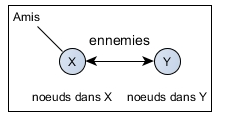
\includegraphics[width=0.5\textwidth]{images/22_amis-ennemies2.png}
\end{figure}

Si un graphe complet est équilibré, alors:

\begin{enumerate}

\item toutes les paires sont amies

\item on peut diviser les nœuds en deux groupes X et Y, tel que X et Y chacun contient des amis mutuels et chaque membre de X est ennemi de chaque membre de Y comme représenté à la figure : \ref{groupami}.

\end{enumerate}

\subsubsection*{Preuve:}

\begin{itemize}\renewcommand\labelitemi{\textbullet}

\item graphe complet, annoté $+,-$

\item graphe équilibré

\begin{enumerate}

\item si aucun lien négatif: (1)

\item sinon il existe un lien négatif

\end{enumerate}

\item prenons un nœud A quelconque

\item Définissons:

\begin{enumerate}

\item $X = A + $ tous ses amis
\item $Y = $ les ennemis de A

\end{enumerate}

\item Est-ce que X et Y satisfont la condition du théorème?
\end{itemize}

\subsubsection*{A démontrer:}


\begin{enumerate}

\item chaque paire dans X = amis

\item chaque paire dans Y = amis

\item chaque nœud de X est ennemi de chaque nœud de Y

\end{enumerate}


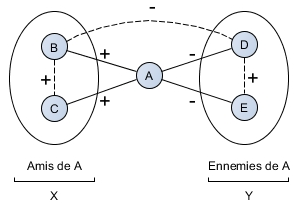
\includegraphics[scale=1]{images/22_amis-ennemies.png}

\subsubsection*{Exemple 1}

On peut retrouver ce type de comportement de graphe dans les relations internationales : lors de la séparation du Bangladesh au Pakistan en 1972, on a assisté à un surprenant soutien des États-Unis pour le Pakistan alors que celui-ci n'était pas un allié des Américains. 
\paragraph{Explication} 
Comme indiqué dans la figure \ref{paysconflit}, les USA désiraient se rapprocher de la Chine, pour y arriver, ils ont analysé les relations des différents pays de la région. Ils ont ainsi constaté que la Chine avait des ennemis communs avec le Pakistan. Un rapprochement avec le Pakistan lui permettait de rentrer dans le groupe des amis de la Chine.


\begin{figure}[h!]
\label{groupami}
\label{paysconflit}
\caption{Relation lors de l'indépendance du Bangladesh}
\centering
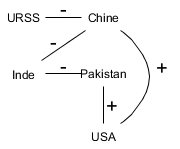
\includegraphics[scale=1]{images/22_pays-conflit.png}
\end{figure}
\paragraph{}
Une autre approche de ce conflit peut être réalisée d'un point de vue de la Chine : 
\begin{itemize}

\item Vietnam du Nord $\overset{+}{\longleftrightarrow}$ Inde

\item Pakistan $\overset{-}{\longleftrightarrow}$ pays du bloc EST

\item Chine : vote l'abolition du Bangladesh à l'ONU

\end{itemize}

\subsubsection*{Exemple 2}
Un autre exemple de ce jeu diplomatique est donné à la figure 55 du livre de référence et représente le jeu des alliances des grandes puissances européennes à la veille de la Première Guerre mondiale. 
\paragraph{}
 On assiste à un équilibrage du graphe des relations avec des pays qui changent continuellement d'alliés jusqu'au moment de la triple entente et de la triple alliance qui sépara tous les pays d'Europe en deux camps ennemis.

\subsubsection*{Exemple 3}
Dans ce troisième exemple, on touche directement les réseaux sociaux tel que Facebook et Twitter où il existe des relations \textit{Like ou Trust} et \textit{Dislike ou Distrust} dont les utilisateurs peuvent se servir pour juger le contenu des autres.
\paragraph{}
Le classement de produits y est libre: un utilisateur est libre d'avoir des opinions positives (+) ou négatives (-) sur les autres


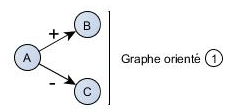
\includegraphics[scale=1]{images/22_graphe-oriente.png}

\subsubsection*{Transitivité}  

Il est intéressant de savoir si les relations sont transitives ou non, autrement dit si A croit en B et que B croit en C, A croira-t-il en C?
\begin{align*}
A \overset{trust}{\longrightarrow} B \overset{trust}{\longrightarrow} C \overset{?}{\longrightarrow} A \overset{trust}{\longrightarrow} C
\end{align*}

Ou alors, si A n'a pas confiance en B et que B n'a pas confiance en C, est-ce que A aura alors confiance en C ou non?


\begin{align*}
A \overset{distrust}{\longrightarrow} B \overset{distrust}{\longrightarrow} C \overset{?}{\longrightarrow} &A \overset{trust}{\longrightarrow} C\\
&A \overset{distrust}{\longrightarrow} C
\end{align*}

Finalement, tout est possible selon le cas rencontré : 
\begin{itemize}
\item Si le trust signifie une relation d'amitié, la transitivité sera respectée. 
\item Si le trust indique une confiance sur l’opinion, la transitivité ne peut être respectée. 
\item Si par contre trust en une proximité dans les opinions politiques, un rapprochement de A et C est probable. 
\end{itemize}


\paragraph{Conclusion :}La théorie de l'équilibre structurel sera gérée selon le cas




\subsection{Équilibre structurel faible}
L'équilibre structurel faible, à l'instar de l'équilibre structurel fort, se base sur la
notion de stabilité des triangles du graphe. Mais contrairement à l'équilibre fort, on ajoute deux cas instables   

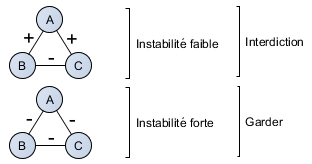
\includegraphics[scale=1]{images/22_Instabilite.png}

Un graphe complet annoté est faiblement équilibré si:
\begin{itemize}
\item aucun triplet n'est $++-$;
\item tous les triplets sont de type $+++, +--, ---$. 
\end{itemize}
\paragraph{}
L'équilibre faible permet une structure \textbf{multipolaire}.

\begin{figure}[h!]
\label{fig:multipolaire}
\caption{Structure multipolaire}
\centering
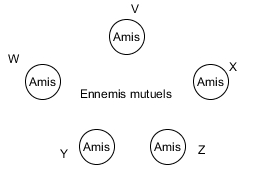
\includegraphics[scale=1]{images/22_etoile-amis.png}
\end{figure}



\subsubsection*{Théorème d'équilibre pour l'équilibre faible}

Si graphe complet annoté est faiblement équilibré, alors on peut diviser ses nœuds en groupes :

\begin{itemize}


\item dans un groupe: amis

\item autre groupe: ennemis

\end{itemize}

\paragraph{Preuve : } \textit{(analogue à la preuve sur l'équilibre structurel)}


\begin{enumerate}

\item Nœud A + tous ses amis appartiennent au groupe X \\
$\to$ amis mutuels, car ($+++$).

\item A $+$ ses amis sont ennemis avec tous les autres.

\item Enlever A $+$ ses amis : nouveau graphe.\\
$\to$ raisonnement récursif

\end{enumerate}
